% !TEX program = xelatex

\documentclass[]{beamer}

\usepackage{xltxtra} 
\usetheme{focus}
\XeTeXlinebreaklocale "th_TH"
\usepackage{fontspec}
\defaultfontfeatures{Mapping=tex-text,Scale=MatchLowercase}
% \setmonofont{Tlwg Typist}
\usepackage{listings}
\usepackage{color}

\definecolor{codegreen}{rgb}{0,0.6,0}
\definecolor{codegray}{rgb}{0.5,0.5,0.5}
\definecolor{codepurple}{rgb}{0.58,0,0.82}
\definecolor{backcolour}{rgb}{0.95,0.95,0.92}

\lstdefinestyle{codeblock}{
    backgroundcolor=\color{backcolour},   
    commentstyle=\color{codegreen},
    keywordstyle=\color{magenta},
    numberstyle=\tiny\color{codegray},
    stringstyle=\color{codepurple},
    basicstyle=\footnotesize,
    breakatwhitespace=false,         
    breaklines=true,                 
    captionpos=b,                    
    keepspaces=true,                 
    numbers=left,                    
    numbersep=5pt,                  
    showspaces=false,                
    showstringspaces=false,
    showtabs=false,                  
    tabsize=4
}
\lstset{style=codeblock}

\usepackage{smartdiagram}

\title{Intro to Machine Learning}
\subtitle{Knowledge Sharing for CPE/SKE students}
\author{Sirakorn Lamyai}
\institute{Student, Kasetsart U.}
\date{\today}
\begin{document}

\begin{frame}
	\titlepage
\end{frame}

\begin{frame}
	\frametitle{Outline}
	\tableofcontents
\end{frame}

\section{Introduction to Machine Learning}

\subsection{What is Machine Learning?}

\begin{frame}
	\frametitle{What is Machine Learning?}
	\pause
	\begin{figure}
		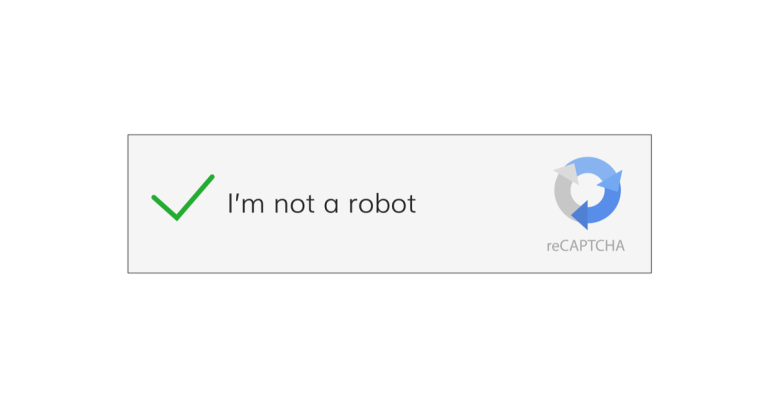
\includegraphics[scale=0.4]{imgs/recaptcha.png}
	\end{figure}
	\begin{itemize}
		\pause
		\item This is Recaptcha.
		      \begin{itemize}
			      \pause
			      \item Recaptcha helps stop millions of spam a day.
			            \pause
			      \item In some old days, we have to type Captcha texts to distinguish ourself from bots.
			            \pause
			      \item How is it possible that with a single click, an automated system can distinguish bots from humans?
		      \end{itemize}
	\end{itemize}
\end{frame}

\subsubsection{Traditional programming approach}

\begin{frame}
	\frametitle{Traditional programming approach}
	\begin{center}
		\smartdiagram[circular diagram]{Analyse, Algorithm, Test, Improve, Repeat}
	\end{center}
\end{frame}


\subsubsection{Machine learning approach}

\begin{frame}
	\frametitle{Machine learning approach}
	\begin{center}
		\smartdiagram[circular diagram]{Analyse, Machine Learning, Validation, Improve, Repeat}
	\end{center}
\end{frame}

\begin{frame}
	\frametitle{In other words...}
	\begin{center}
		Machine Learning \\
		\onslide<2-> \huge = Data + Data analysis algorithm \\
		\onslide<3-> \Huge = Adapt to change
	\end{center}
\end{frame}

\section{Machine Learning Problems}

\begin{frame}
	\frametitle{Types of Machine Learning problems}
	\begin{enumerate}
		\item<2-> Supervised learning
		\item<3-> Unsupervised learning
		\item<4-> Reinforcement learning
	\end{enumerate}
\end{frame}

\subsection{Supervised learning}

\begin{frame}
	\frametitle{Supervised learning}
	\begin{columns}
		\column{0.5\textwidth}
			\begin{figure}
				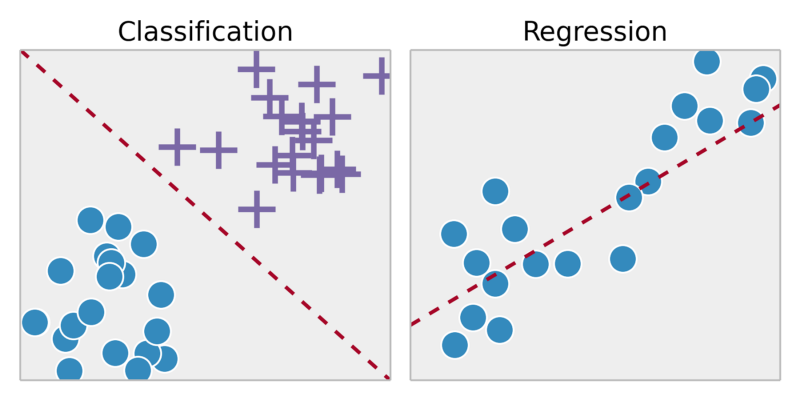
\includegraphics[width=1.0\textwidth]{imgs/supervised_learning.png}
			\end{figure}
		\column{0.5\textwidth}
			\begin{itemize}
				\item<2-> Given a \textbf{training set} for the data, find a \textbf{model} to \textbf{generalise} well to \textbf{unseen} data.
				\item<3-> Two main supervised learning problems
				\begin{itemize}
					\item<4-> Classification: On the discrete data
					\item<5-> Regression: On the continuous data
				\end{itemize}
				\item<6-> Example problems: Spam E-mail detection, Facial recognition
			\end{itemize}
	\end{columns}
\end{frame}

\subsection{Unsupervised learning}

\begin{frame}
	\frametitle{Unsupervised learning}
	\begin{columns}
		\column{0.5\textwidth}
			\begin{figure}
				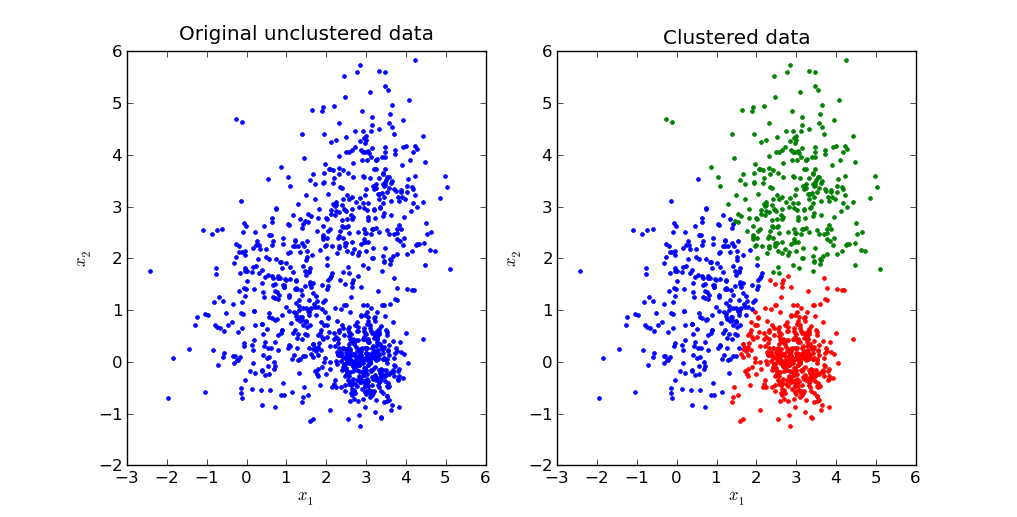
\includegraphics[width=1.0\textwidth]{imgs/kmeans.png}
			\end{figure}
		\column{0.5\textwidth}
			\begin{itemize}
				\item<2-> Discover \textbf{hidden} structure in \textbf{non-labelled} data.
				\item<3-> Example: Clustering, Generative models
			\end{itemize}
	\end{columns}
\end{frame}

\subsection{Reinforcement learning}

\begin{frame}
	\frametitle{Reinforcement learning}
	\begin{figure}
		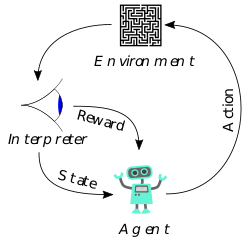
\includegraphics[scale=.7]{imgs/reinforcement_learning.png}
	\end{figure}
\end{frame}

\section{Model}

\begin{frame}
	\frametitle{Model}
	\begin{itemize}
		\item<2-> A result of the combination between...
		      \begin{itemize}
			      \item<3-> a \textbf{method} to recognise the data, and
			      \item<4-> \textbf{sample datas} for such the method
		      \end{itemize}
	\end{itemize}
\end{frame}


\begin{frame}
	\frametitle{Model}
	\begin{columns}
		\column<2->{0.5\textwidth}
		\begin{figure}
			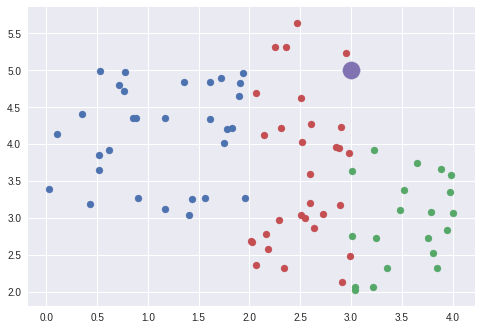
\includegraphics[scale=.3]{imgs/simple_knn.png}
		\end{figure}
		\column<3->{0.5\textwidth}
		Determine which group should the purple dot be in (red/green/blue) by \textbf{checking the colour of its nearest dot.}
	\end{columns}
	\begin{columns}
		\column{0.5\textwidth}
		\begin{center}
			\Large Data
		\end{center}
		\column{0.5\textwidth}
		\begin{center}
			\Large Method
		\end{center}
	\end{columns}
\end{frame}

\begin{frame}
    \frametitle{Beginning with our first model}
    \begin{itemize}
        \item<2-> We're going to write our \textbf{first own} machine learning algorithm called \textbf{$k$-Nearest Neighbour} ($k$NN)
        \begin{itemize}
            \item<3-> $k$-NN is known to be very simple, with its concept as
        \end{itemize}
    \end{itemize}
    \onslide<4->
    \begin{block}{$k$-NN algorithm}
        To classify label of a data point, get $k$ nearest data points to the data point, and select the major label among those data points.
    \end{block}
\end{frame}

\subsection{A good model}
\begin{frame}
	\begin{center}
		{\Huge Good model?}\\
	\end{center}
\end{frame}

\begin{frame}
	\frametitle{Good model}
	\begin{figure}
		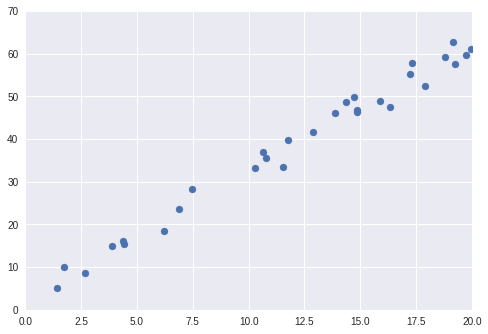
\includegraphics[scale=.4]{imgs/linreg_1.png}
	\end{figure}
	\begin{center}
		How should we \textit{draw} the line to predict this data?
	\end{center}
\end{frame}

\begin{frame}
	\frametitle{Good model}
	\begin{figure}
		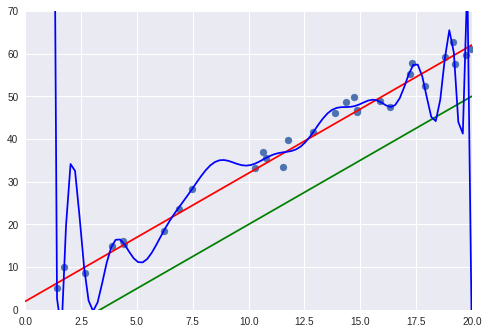
\includegraphics[scale=.4]{imgs/linreg_2.png}
	\end{figure}
	\begin{center}
		Blue, red, or green line?
	\end{center}
\end{frame}

\subsubsection{Overfitting and underfitting}
\begin{frame}
	\frametitle{Overfitting and underfitting}
	\begin{columns}
		\column{0.5\textwidth}
		\begin{figure}
			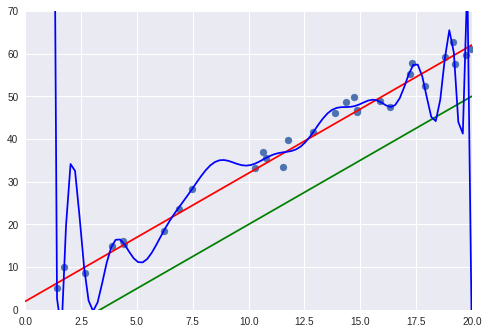
\includegraphics[scale=.3]{imgs/linreg_2.png}
		\end{figure}
		\column{0.5\textwidth}
		\begin{enumerate}
			\item<2-> Underfitting
			      \begin{itemize}
				      \item<3-> Our model \textbf{fails to know the data's trends}
				      \item<4-> Resulting in failure to predict further data
			      \end{itemize}
			\item<5-> Overfitting
			      \begin{itemize}
				      \item<6-> Our model \textbf{memorise instead of generalise}
				      \item<7-> Resulting in failure to catch the trend
			      \end{itemize}
		\end{enumerate}
	\end{columns}
\end{frame}

\begin{frame}
	\begin{center}
		{\LARGE Good model must \textbf{generalise}}\\
	\end{center}
\end{frame}

\end{document}